\chapter{Leonard Bloomfield}
\label{ch.bloomfield}

Few figures in the history of linguistics stand out so dramatically as
incarnations of their time and place as does \name{Leonard}{Bloomfield}, the
symbol of theoretical thought about language in North America from the
late 1930s through the
1950s.\footnote{\citet{hockett70:bloomfield.anthology} provides a
  collection of {\Bloomfield}'s important papers and obituaries, with
  notes and commentary; \citet{fought99:bloomfield} offers a
  comprehensive collection of analyses of {\Bloomfield}'s life and
  work. The centenary of {\Bloomfield}'s birth in 1987 produced a special
  commemorative session at the LSA meeting and a number of reviews,
  several of which were collected as volume 14, numbers 1/2 of the
  journal \textsl{Historiographia Linguistica} and subsequently
  published as
  \citealt{hall87:bloomfield.essays}. \citet{hall90:bloomfield.bio}
  provides additional information in a useful, if somewhat
  idiosyncratic, biography, and \citet{hockett99:bloomfield.bio} gives
  further biographical remarks.}  Most of the development of
linguistic theory in America during this period is usually attributed
either to his own work or to the work which his students and followers
carried out in the name of his views. As will become apparent in
chapter~\ref{ch.structuralists}, a good deal of what went on in the
self-consciously `post-Bloomfieldian' period was not particularly
close to {\Bloomfield}'s own views; but many nonetheless felt that a
scientific approach to language could be largely identified with the
task of working out {\Bloomfield}'s theoretical notions. Especially from
the point of view of those elsewhere, American linguistics in this
period basically was Bloomfieldian linguistics.

Of course, {\Bloomfield} was by no means the only linguist of note in
North America during this period.  As shown in the previous chapter,
his activity during the 1930s overlapped with that of {\Sapir}, who was a
major figure before {\Bloomfield}'s work was generally known; for that
matter, {\Boas} was still alive when {\Bloomfield} was working, and indeed
all three of these figures worked together in some cases. Some of the
reasons for {\Bloomfield}'s gradual ascendancy have already been noted:
probably a central consideration was his identification with the
growth of linguistics as an autonomous scientific discipline. {\Boas} and
{\Sapir} had established an independent position identified with the
study of language in North America, but their work was largely thought
of as a tradition within the field of \isi{anthropology}. {\Bloomfield}, on the
other hand, was closely identified with the rise of a distinct
professional field of linguistics.

One factor in this identification was his prominence in the
development of the distinctive institutions of the new field. He was
one of those (together with \name{George M.}{Bolling} and \name{Edgar}{Sturtevant}) who
wrote the ``Call'' for the formation of a linguistic society in the
United States, as well as the author of the lead article ``Why a
Linguistic Society?'' \citep{bloomfield1925:why.lsa} in the first issue
of \textsl{Language}. He participated enthusiastically in the
activities of the society, and was its president in
1935.\footnote{\citet{murray91:lsa} provides an account of the origins
  and activities of the LSA in its first 25 years; \citet{hill91:lsa}
  picks up the story and carries it on through 1968.} He taught
several times at the \isi{Linguistic Institute}, including introductory
courses that served as the focus of attention at this annual event. To
appreciate this, we must recall that the institute served a much more
important service function in its early days, before linguistics was
taught \emph{per se} in more than a very few universities; and the
introductory course taught at the institute constituted virtually the
only way for many to gain an idea of the content of the discipline.

Another relevant factor was the constant {stress} in {\Bloomfield}'s
writing on the independence of linguistics from other fields, and the
consequent necessity to develop its autonomous assumptions in a
rigorous way from minimal basic principles. This he felt to be
essential to the scientific status of the study of language; and the
alignment of these views with the philosophical and scientific tenor
of the times made him a natural candidate for the status of
theoretical spokesman for the new discipline. As early as 1926, when
he published his ``Set of Postulates for the Science of Language''
\citep{bloomfield26:postulates}, {\Bloomfield} had staked out the issue
of `scientific rigor' as peculiarly his own.

Subsequently, his text \textsl{Language} \citep{bloomfield:lg} served
as the introduction to the field for more than one generation of
students, and this impact was reinforced by his popular and effective
teaching at the LSA's summer Linguistic Institutes. Though he had few
students himself, his role in the organization of the army's Intensive
Language Program during World War II further reinforced his influence
on the most active and aggressive of younger scholars, who would
dominate the emerging field after the war. Taken together with the
genuine novelty of his theoretical views, these factors help to
explain why, as linguistics took on a clearer professional identity in
the United States during the 1930s and 1940s, a large part of that
identity was based explicitly on the work of {\Bloomfield}.

\section{Bloomfield's life and career}

{\Bloomfield} was born in Chicago in 1887, and grew up there and in
Elkhart Lake, Wisconsin, where his family had purchased a resort
hotel. After returning to Chicago for High School, in 1903 he went to
Harvard, where, by virtue of some extra credit awarded on entrance, he
was able to earn a BA by 1906. He then went on to the University of
Wisconsin as a teaching assistant and graduate student but not a
candidate for a degree.  His meeting with \name{Eduard}{Prokosch} on his
initial visit to Wisconsin apparently helped him to settle on \ili{Germanic}
and linguistics as a career. In 1908 he left Wisconsin for the
University of Chicago, from which institution he received his
doctorate in 1909 for his thesis ``A Semasiologic Differentiation in
\ili{Germanic} Secondary Ablaut'' (published as
\citealt{bloomfield09:thesis1,bloomfield10:thesis2})

This work is essentially a series of 249 families of words within
\ili{Germanic}, each of which shows a pattern of (innovated) Ablautlike
vocalic \isi{variation} which is utilized for essentially sound-symbolic
purposes. These sets are preceded by an introduction to the nature of
the phenomenon and some remarks on the correlation between particular
vocalisms and their gross semantic spheres. Though clearly addressing
issues of some generality, it is also an excellent example of the
detailed investigation of particular topics which marked {\Bloomfield}'s
research in \ili{Germanic} and, later, his study of \ili{Algonquian} languages.

In 1909, he began his teaching career at the University of Cincinnati,
and in 1910 moved to the University of Illinois. In those years (and
in fact for most of his academic life) his major teaching
responsibility was \ili{German}—often the most basic courses. This
occupation with elementary language teaching was by no means just a
painful necessity for {\Bloomfield}: he concerned himself with problems
of language pedagogy throughout his life, and spent much energy on
bitter criticism of the attitudes of `educationists' whose methods he
found sadly wanting in light of modern linguistic understanding. Among
his less-known writings are to be found a \textsl{First {German} Book}
from 1923, as well as an {English} reader for elementary schools, which
was organized to minimize the trauma of the idiosyncrasies of \ili{English}
\isi{orthography} for beginning readers. The strictly linguistic interest of
these works, alas, is not as great as the commitment they show on his
part to problems of linguistic pedagogy.

Told by his Chairman that he could only be eligible for promotion if
he had studied in Germany, he spent 1913-14 in {Leipzig} and Göttingen,
improving his background in \ili{Indo-European}, \ili{Sanskrit}, and related
studies. His preparation in these areas was already quite substantial
thanks to work with {\Prokosch} and others at Wisconsin, and to his year
at Chicago; it is also probably not irrelevant that his uncle 
\name{Maurice}{Bloomfield} was a distinguished Sanskritist (and the second president
of the {Linguistic Society of America}). During this year he studied
with {\Leskien} and {\Brugmann} among others. Although such study in Germany
was a necessary rite of passage for those who wanted to advance in the
academic profession of \ili{Germanic} studies, {\Bloomfield} may have chosen an
unfortunate time to pursue this field. The outbreak of the first World
War radically reduced interest in \ili{German} in the United States.

Conventional wisdom has it that a greatly reduced number of students
in \ili{German} classes lessened {\Bloomfield}'s teaching load and provided him
with the spare time needed to take up other studies. Firm statistics
are not available, but a 1939 letter from him quoted by
\citet[41]{hall90:bloomfield.bio} would seem to contradict this:
\begin{quotation}
  The administrative treatment of \ili{German} has always seemed
  inexplicable to me. Way back in 1917 when I was temporarily for the
  first time in charge of the Department, our sections were closed
  early in the Autumn registration, and we estimated that we had
  turned away as many students as we had admitted. When I made a
  protest, I got the obviously incorrect answer that budgetary
  considerations forbade our giving more sections---this of the one
  phase of our work that earns money for the University!
\end{quotation}
Something other than an abundance of free time, then, probably
motivated him in 1915-16 to take up his first real fieldwork—on
Tagalog, with a native speaker who was a student at Illinois. The
resulting analysis of this language \citep{bloomfield16:tagalog},
even based as it was on limited elicitation from a single speaker, is
widely considered one of the best and most complete descriptions ever
produced of an Austronesian language, despite difficulties resulting
from {\Bloomfield}'s conscious avoidance of traditional grammatical
terminology.

In 1914 {\Bloomfield} had published his first major work, \textsl{An
  Introduction to the Study of Language}
\citep{bloomfield14:introduction}. This book, based on \name{Wilhelm}{Wundt}'s views
on the \isi{psychological basis of language}, was well received, and
(though not particularly revolutionary) furnishes an excellently
organized and presented view of the state of general linguistics at
the time. In connection with this book, it is interesting to note
something that was already becoming a particularly American trait in
writing about language. More than one of his reviewers found
{\Bloomfield}'s examples from a wide variety of `exotic' languages
unconvincing (because unfamiliar), and took him to task for appealing
to these rather than sticking to the well-known members of the
{Indo-European} family.

In 1921, he was offered a promotion from assistant professor at
Illinois (where unconfirmed rumor has it that he was in fact denied
tenure) to full professor at Ohio State University. It seems this
offer was made largely on the initiative of the classicist 
\name{George M.}{Bolling}, who would be a close colleague at Ohio State and
collaborate in initiating the call for the formation of a linguistic
society. He naturally accepted the call to Columbus, where he finally
had the opportunity to teach some linguistics, although his primary
responsibility was still in \ili{German}. A more important aspect of his
years at Ohio State than his actual teaching there, though, was
probably his association with the psychologist \name{Alfred P.}{Weiss}, whose
behaviorist views (in conjunction with more general scientific
influences of the times) quickly came to replace completely
{\Bloomfield}'s earlier acceptance of Wundt\ia{Wundt, Wilhelm}.

In 1927, {\Bloomfield} was invited to the University of Chicago to
succeed his former mentor \name{Francis A.}{Wood} in the chair of \ili{Germanic}
Philology. It was during this period that he and {\Sapir} were colleagues
(albeit in different departments, and somewhat uneasy
acquaintances). Most of the students in linguistics at Chicago were
working with {\Sapir}, and although {\Bloomfield} again taught some
linguistics, his main responsibilities were still in \ili{Germanic}
philology.

\begin{wrapfigure}{r}{.35\textwidth}
  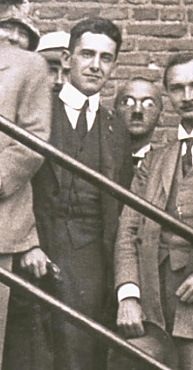
\includegraphics[width=.95\textwidth]{figures/bloomfield_1924.jpg}
  \caption{Leonard Bloomfield at the International Congress of
    Americanists, The Hague, 1924 (Alice Bloomfield obscured, upper left)}
  \label{fig:ch.bloomfield.bloomfield_1924}
\end{wrapfigure}
During his time at Chicago, he became increasingly well known as a
general linguist. Though he continued to work in \ili{Germanic}, he had
begun fieldwork on languages of the {Algonquian} family. As early as
1920, he spent time on the Menominee reservation near his parents'
hotel in Elkhart Lake, two summers of field study that would serve as
the basis for his later extensive analyses of \ili{Algonquian} beginning
with \citealt{bloomfield24:menomini}. His field work was supported for
one summer (in 1925, working with Sweet Grass and other Cree people in
Saskatchewan) by {\Sapir} and the Canadian Department of Mines; it is
perhaps interesting to note that {\Sapir}, who did not know {\Bloomfield} at
all directly, was initially hesitant about this appointment, fearing
that {\Bloomfield} might be too much of a philologist to make a good
fieldworker.

His \ili{Algonquian} work was to occupy much of his attention for the rest
of his scholarly life, covering a number of the languages of the
family in considerable depth. It also served as the basis of what
would become a paradigmatic demonstration of the power of the
comparative method, and of its applicability to unwritten languages as
well as to those with a long period of attestation: a consonant
cluster reconstructed by {\Bloomfield} for proto-\ili{Algonquian} on the basis
of a single set of cognates was subsequently confirmed by the
discovery of unique reflexes in other, previously unstudied (or poorly
described) dialects of the family. As a validation of the general
assumptions of neogrammarian theories about \isi{historical change}, this
result took on nearly the same value as did the discovery of \ili{Hittite}
for Saussure's posited abstract \textsl{coéfficients sonantiques} (the
iaryngeals') as discussed in chapter~\ref{ch.saussure_life}.

Especially as his book \textsl{Language} \citep{bloomfield:lg} became
well known in the late 1930s, {\Bloomfield} became a truly major figure
in American linguistics. In 1940 he received an offer to replace the
recently deceased {\Sapir} as Sterling Professor of Linguistics at
Yale. Discontented with the lack of support for his scientific work at
Chicago, due to administrative obligations, the ongoing need to teach
in \ili{Germanic}, and the lack of secretarial help, he found this tempting,
although his ties to Chicago were close. Some discussion with the
university's administration persuaded him that Chicago was not really
interested in doing much to improve his
situation,\footnote{\citet[59ff.]{hall90:bloomfield.bio} quotes
  correspondence from files at the University of Chicago which only
  became available for examination in 1989 to argue that
  administrators there, especially Dean \name{Richard}{McKeon}, were
  sympathetic to {\Bloomfield}'s case and would have worked to keep him
  there. As I read this material, I find little substantive support
  for this position, and no evidence that any concrete steps were
  being taken to address the issues {\Bloomfield} raised. Others may feel
  differently. In any event, {\Bloomfield} himself was not persuaded, and
  decided to leave.} and he accepted the Call to Yale.

\begin{wrapfigure}{r}{.4\textwidth}
  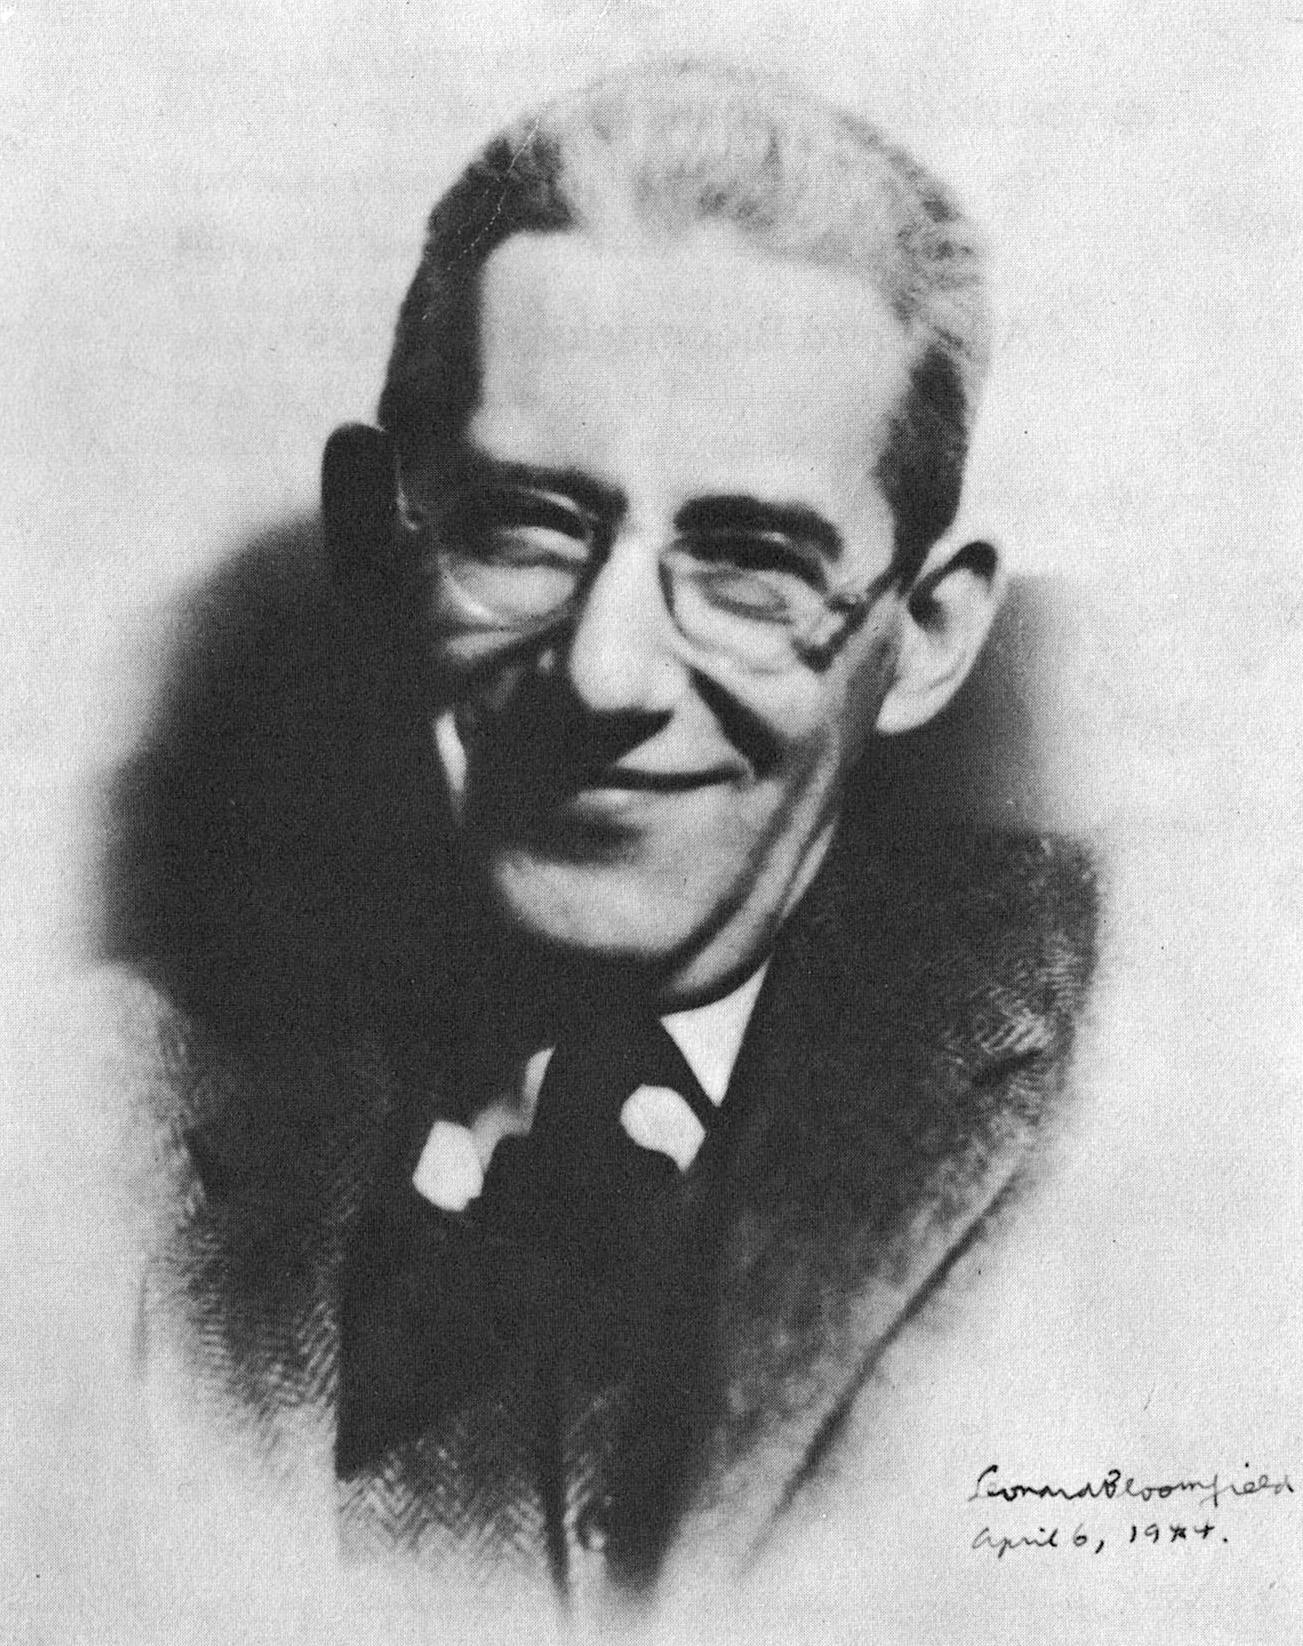
\includegraphics[width=.95\textwidth]{figures/bloomfield_1944.jpg}
  \caption{Leonard Bloomfield (1944)}
  \label{fig:ch.bloomfield.bloomfield_1944}
\end{wrapfigure}
At Yale, it was expected that he would be able to devote all of his
attention to general linguistics; but unfortunately he never really
settled in at Yale. His wife Alice\ia{Bloomfield, Alice} had been extremely attached to life
in Chicago, and suffered a complete breakdown when obliged to move to
New Haven. She never really recovered, and spent the rest of her life
in and out of sanitariums. The family never settled in their new city,
and lived in a hotel for most of the time until {\Bloomfield} became
incapacitated and they came to live with friends. Needless to say,
these disruptions contributed to {\Bloomfield}'s unhappiness about his
general circumstances.

The outbreak of the second World War disrupted normal academic life,
and much of {\Bloomfield}'s energy from 1942 to 1945 was devoted to the
practical problems of the US Army's Intensive Language Program. A
great many linguists, from Yale and elsewhere, were recruited to
produce materials for the teaching of a variety of strategically
significant languages. One of these was \ili{Russian}: after {\Trager} produced
a set of materials containing a great many inaccuracies with respect
to the standard language, an effort that was sharply criticized by
{\Jakobson}, {\Bloomfield} took this over. He also produced two stages of
materials for Dutch. A number of prominent descriptive linguists,
including Yale faculty, were engaged in work in New York at 1965
Broadway \citep{hall91:165broadway}.

\begin{wrapfigure}{r}{.4\textwidth}
  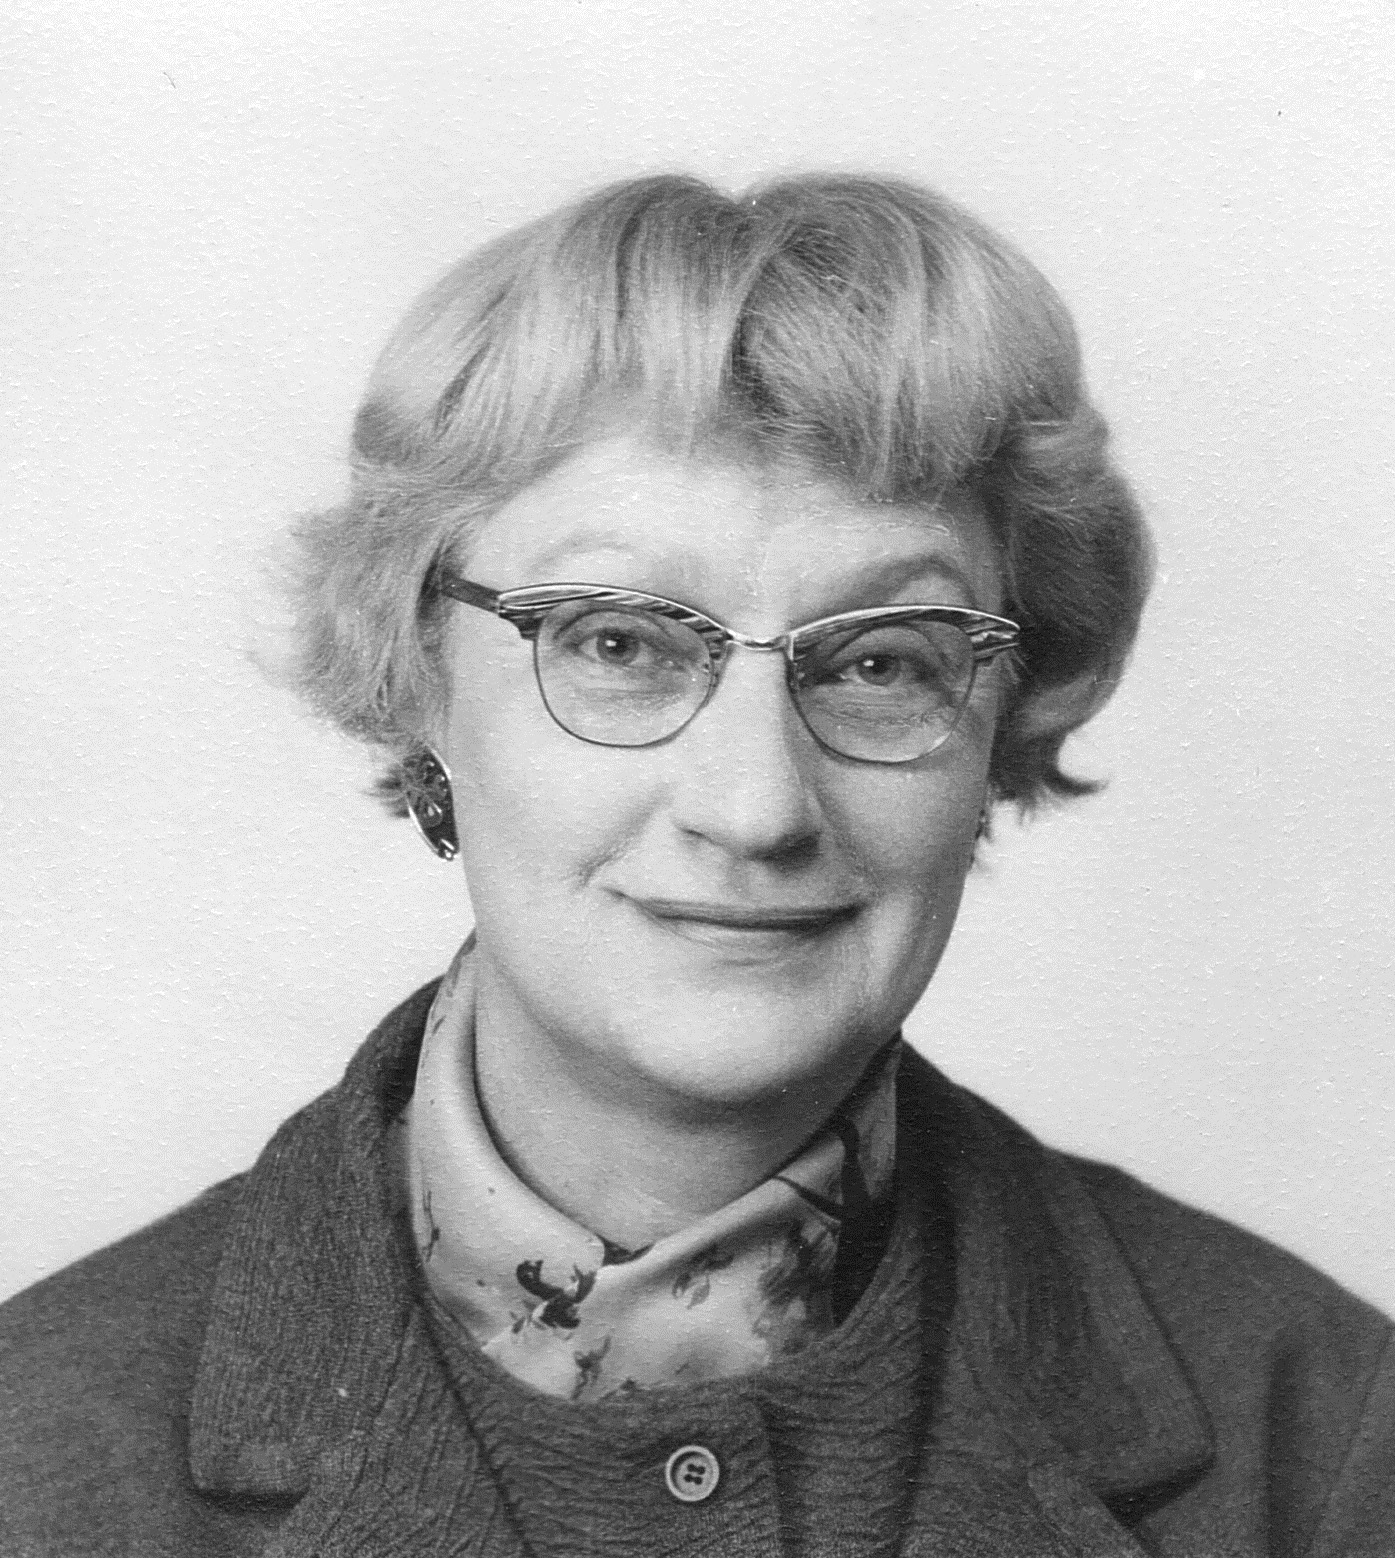
\includegraphics[width=.95\textwidth]{figures/Mary-Haas-aps.jpg}
  \caption{Mary Haas}
  \label{fig:ch.bloomfield.haas_aps}
\end{wrapfigure}
Elsewhere, \name{Murray}{Emeneau} was assigned Vietnamese and Mary {\Haas} was
given Thai, a project she took up with great seriousness, starting
with two years of study at the University of Michigan before joining
{\Kroeber}'s program at Berkeley. This effort resulted in her shifting
her attention from the northwest coast and southeast of North America
to Southeast Asia for much of the remainder of her career, an area in
which she became one of the world's leading specialists.

In 1946, {\Bloomfield} suffered a disastrous stroke, from which he never
really recovered. Though he lived until 1949, he was essentially
unable to do further scholarly work during this period; and at his
death left a number of projects (including his major grammar of
\ili{Menomini}, as well as a lexicon of the language, and a grammar of
Eastern Ojibwa) unfinished. Much of this material has since been
prepared for publication, largely through the efforts of Charles
{\Hockett}.

\section{Bloomfield's view of language, linguistics, and psychology}

{\Bloomfield}'s opinions about the nature of language and the procedure
by which it should be investigated marked a major reorientation in
American linguistics, but we cannot examine here all of the issues
raised by his position. A substantial literature already exists in
this area (see, e.g., \citet{hockett70:bloomfield.anthology};
\citet{esper68:bloomfield};\citet{teeter69:bloomfield};
\citet{stark72:bloomfield}; \citet{hymes.fought81:structuralism} and
numerous references cited there and more recently in
\citet{fought99:bloomfield}), and a survey of it would take us far
afield. On the other hand, one central issue is directly relevant to
establishing the bases of {\Bloomfield}'s specifically phonological views
and must be at least sketched. This is the question of his attitude
toward psychology, and especially the role of `\isi{meaning}' in linguistic
structure. In this connection we treat briefly some aspects of the
philosophy of science that are dealt with explicitly in his writings.

\citet{bloomfield14:introduction}, his first work in general
linguistics, starts from two general sets of premises: those of
Wundt\ia{Wundt, Wilhelm}'s \emph{Volkerpsychologie} with respect to the central part
played by psychological considerations in understanding the nature of
language, and those of his Neogrammarian teachers concerning the
mechanical nature of linguistic change and the possibility of a
rigorous account of its operation. His enthusiasm for Neogrammarian
theories never weakened, and in fact he saw as one of the advantages
of the overall position that he later developed the extent to which it
allowed him to rationalize the underlying assumptions of the
Neogrammarians.

Within a fairly short time, however, whatever doubts he may earlier
have had about the explanatory value of Wundtian psychology were
replaced by an ardent commitment to behaviorist (or ``mechanist,'' as he
preferred to put it) assumptions about the nature of the human
mind. This {change} in outlook appears quite clearly in
\citealt{bloomfield26:postulates}, his ``Postulates,'' where he
attempted to state the foundational assumptions of linguistic study in
as explicit a way as possible.

The influence of his acquaintance and close friendship with {\Weiss} at
Ohio State is clearly evident here, at least on the surface: the
``Postulates'' are intended to be modeled on {\Weiss}' set of postulates
for psychology, though in fact the resemblance is not very close
({\Bloomfield}'s postulates in fact resemble the axiomatization of
linguistics attempted in Pāṇini's
grammar\footnote{\citet{rogers87:bloomfield.panini} discusses the
  influence on {\Bloomfield}'s work of his knowledge of Pāṇini, dating to
  his study with \name{Jakob}{Wackernagel} in Göttingen.}  more than they do
{\Weiss}'s postulates for psychology). More importantly, no doubt, the
terminology of reference to psychological factors is wholeheartedly
behaviorist in orientation (as when the meanings of utterances are
defined as their ``corresponding stimulus-reaction features'').

The central factor underlying both his maintenance of Neogrammarian
assumptions about change and the shift in his point of view on
psychology was undoubtedly {\Bloomfield}'s passion for scientific
{explanation} based solely on propositions relating observable factors
and influences by principles of logic and \isi{mathematics} alone, a product
of the times. Throughout his career, he would again and again ridicule
appeals in the supposedly scientific linguistic literature to
`mentalistic' explanations. It is important to understand that, by
this term, he did not mean (as often understood by subsequent
commentators) to deny the existence of human mental life. Rather, he
intended to reject the notion that a deterministic, causative role is
played in shaping linguistic (or other) phenomena by a mysterious and
unobservable entity (``mind''), whose principal property is its
non-obedience to the normal laws of physical structure or to any other
discoverable system.

There are, of course, conceptions of the nature of mental and
cognitive activity that allow such systems to be taken seriously as
the objects of non-mystical investigation, without requiring (as early
behaviorists did) that they be reduced to special cases of the
activity of other physical organs. {\Bloomfield}, however, saw appeals to
a distinctive mental structure underlying language not as attempts to
elucidate the special nature of this cognitive system but, rather, as
an attempt to evade rational {explanation} for the facts of
language. Considering the excesses along such lines that had earlier
been committed in the name of a romanticist philosophy of language and
mind, this concern was by no means totally illusory. For {\Bloomfield},
however, the obvious (indeed, only) alternative to anti-rationalist
speculation about the mysteries of the human soul was to deny
scientific existence to anything other than the material embodiment of
mind in a system of nerves and related tissue supporting systematic
patterns of electrical activity.

{\Bloomfield}'s account of mind (and particularly the nature of \isi{meaning},
a linguistic aspect of mind) in his later work such as
\textsl{Language} is thus intended to be founded on factors that are
(at least in theory) observable. The description he gives of \isi{meaning}
is entirely in terms of situation, context, and the disposition of a
speaker to respond in particular ways to particular stimuli. If we
knew every detail of a speaker's history, he suggests, from a complete
description of the composition of his nervous system, internal organs,
etc., at birth through a comprehensive history of all stimuli to which
he was ever exposed, we could in principle know how he would respond
to any particular linguistic stimulus—and the combination of such a
stimulus with its response in a given situation was all {\Bloomfield}
recognized as coherent in the notion of the \isi{meaning} of a linguistic
form. To assume in addition that the form corresponded to an
unobservable `\isi{concept}' internal to the speaker was for {\Bloomfield}
simply anti-scientific mysticism.

{\Bloomfield} thus did not (as he is often portrayed as doing) reject the
notion that linguistic forms have meanings. He did believe, though,
that a satisfactory account of \isi{meaning} would involve an encyclopedic
knowledge of the world and its laws in the most minute detail—a task
obviously going far beyond the scope of linguistics, and in fact
constituting the subject matter of the non-linguistic sciences of
physics, physiology, etc.

It is quite clear that if we examine this account of \isi{meaning} in detail
(without {\Bloomfield}'s \emph{a priori} commitment to purely `mechanist'
foundations for theoretical constructs), it is no more defensible than
the `mystical' view he was attacking. He does not in fact attempt to
give the required description of the \isi{meaning} of any particular
utterance (and more importantly, to go beyond the treatment of
particular utterances on particular occasions to the \isi{meaning} of a
sentence in general, independent of its particular situational
context), but there is every reason to believe that, if he had, he
would have found it essentially a matter of faith to maintain that, at
a sufficiently minute level, there are observable factors which
completely explicate sentence \isi{meaning}. Most of the internal
neurological events and material consequences of previous stimuli that
{\Bloomfield}'s view depends on for its account of mind are as much a
matter of faith on his part as the `mentalist' picture is for others.

In fact, the choice between `\isi{mentalism}' and `\isi{mechanism}' as paths to
the understanding of \isi{meaning} is one between research programs rather
than between concrete propositions or theories. Both views assume that
there is something linguistically relevant (the `meanings' of
linguistic forms and their parts) which must be accounted for; they
differ in the assumptions they make about where to look for a suitable
foundation for this construct. {\Bloomfield} himself considered that only
the mechanistic approach could be defended as scientific; but
interestingly enough, he maintained repeatedly that the choice between
them was, strictly speaking, irrelevant to linguistics.

The reason for this is that linguistics is concerned with the study of
languages as systems that pair \isi{sound and meaning}, and he felt that the
structure of such associations could be investigated even in the
absence of a precise knowledge of just what the sounds and the
meanings are that are paired. Sound and \isi{meaning} enter the construction
of linguistic theories at an absolutely basic level: the ``fundamental
assumption of linguistics,'' first presented in
\citealt{bloomfield26:postulates} and subsequently developed in
several other places (including \textsl{Language}), is that ``in every
speech community some utterances are alike in form and \isi{meaning}''
\citep[78]{bloomfield:lg}. Nonetheless, just what the meanings of
those utterances are (as well as the phonetic details of their
production) need not be known in order to get on with the business of
analyzing the system in which they have \isi{meaning}.

Somewhat paradoxically, then, {\Bloomfield} introduces his view of
linguistic \isi{meaning} only to exorcise the details of it from the
investigation: to claim not that linguistic analysis disregards
\isi{meaning} but that the concrete nature of \isi{meaning} can be reduced to a
postulate, something external to language itself. Strictly speaking,
then (as he argued on various occasions), the issue of mentalist
versus mechanist theories of \isi{meaning} is one that is external to the
development of a theoretical account of the structural properties of
language. In a provocative (if somewhat overstated) image, he likened
the circumstances of his `anti-\isi{mentalism}' to ``a community where nearly
everyone believed that the moon is made of green cheese, [in which]
students who constructed nautical almanacs without reference to
cheese, would have to be designated by some special term, such as
non-cheesists'' \citep[49]{bloomfield44:secondary}.

Meaning, like the moon, is an essential term of theories in the
relevant domain, but the concrete content of either is strictly
speaking an orthogonal issue. Admittedly, {\Bloomfield} felt compelled
(and entitled) to push his own opinions about what \isi{meaning} is and how
it should (and should not) be investigated; but it is noteworthy that
the specific details of his reductionist account play little or no
role in his discussion of other areas of linguistic structure. What
remains is the assumption that utterances (and their parts) have
\isi{meaning}; that linguists as a practical matter know a great deal about
what these meanings are, when they are alike or different, etc.; and
that even if they cannot give a complete scientific account of
individual meanings, their practical knowledge still allows them to
get on with the task of analyzing language, since \isi{meaning} enters the
analysis only in the form of a posited external property of linguistic
forms.

Whether meanings can be successfully treated as outside the scope of
linguistics is an issue quite parallel to that raised by {\Bloomfield}'s
efforts to exclude phonetics in a similar way as an external
discipline. This attempt on his part will be discussed below, where it
is argued that, while the issue is a substantive one, there are good
empirical reasons for including the study of linguistic phonetics
within the science of language (and not only as a branch of physics or
physiology). In the case of the study of \isi{meaning}, however, it must be
admitted that our actual substantive understanding of this area is
sufficiently meager that we are far from being able to develop the
corresponding argument. Fortunately, in a work devoted to phonology,
this issue can be left unresolved.

The independence of linguistics from any particular psychological
assumptions seemed to {\Bloomfield} to be recommended not only by general
methodological considerations but by substantive ones as well. Thus,
psychology is fundamentally the study of the workings of individual
minds; and {\Bloomfield} found it difficult to accept that this could
provide an adequate basis for explaining the workings of an
essentially social phenomenon like language.

More importantly, the posited independence of linguistic mechanisms
provided a basis for an explanatory theory of language change. For
{\Bloomfield}, the overwhelming accomplishment of previous study of
language was the body of results achieved by nineteenth- and early
twentieth-century comparativists concerning the history and
development of languages. These results, in his view, were inseparable
from the assumption of the regularity of \isi{sound change}. In numerous
articles and reviews, he criticized scholars who would admit even as a
marginal possibility the existence of sporadic or incomplete sound
changes, the inhibition of \isi{sound change} by factors such as
onomatopoeia or specialized \isi{meaning}, and other such non-phonetic
influences. Even a single clear instance of such a limitation on the
operation of \isi{sound change} would, he felt, essentially evacuate the
explanatory power of the notion itself, since it would lay open the
possibility that any observed change was due to the operation of
sporadic factors, and not to a clear regularity at all.

This does not mean that {\Bloomfield} recognized only blind phonetic
change as a \isi{mechanism} of linguistic development. In \textsl{Language}
he gives one of the clearest accounts available in the literature of
the workings of mechanisms such as \isi{analogy} and a variety of sorts of
borrowing. The point is that each of these other mechanisms can be
distinguished from \isi{sound change} \emph{per se}, and when these
manifestly distinct categories are set aside, what remains is simply
``\isi{sound change}''—a fully determinate process, which does not fall into
``sporadic'' and ``\isi{regular}'' types. A shift which is validly considered
``\isi{sound change}'' may of course take place only in some specifiable set
of phonetic environments; but this simply indicates that in the
general case, \isi{sound change} consists in the replacement of certain
sound \emph{sequences} by other sound sequences. In particular, it
does not mean that sound changes can affect only a portion of the
vocabulary determined by some extra-phonetic criterion.

Having argued that \isi{sound change} (strictly construed) is an essentially
\isi{regular} process, {\Bloomfield} finds the \isi{explanation} of that fact in the
autonomy of linguistic structure. His reformulation of the classic
Neogrammarian principle (``Sound laws have no exceptions'') is simply
that ``phonemes change'': i.e., that it is possible that the
articulatory implementations of phonemes or their structural
interrelations may be changed, but that when this happens it affects
in identical ways every linguistic form in which the changed \isi{phoneme}
occurs. Since the role of phonemes in particular forms is dependent
only on the nature of the phonemes in question, and not on the
\isi{meaning}, frequency, etc., of the forms themselves, there is no way
that such factors could possibly influence the working of a change
affecting the phonemes. A correct understanding of the independence of
linguistic structure from factors that are properly extra-linguistic
allows for the demystification of the traditional doctrine, and for
its understanding as a genuinely explanatory principle.

It can certainly be argued (as of course it has been) that
{\Bloomfield}'s views on the nature of mental and cognitive organization
were excessively simplistic, and that they cannot form the basis of a
genuinely adequate theory of language. I definitely have no intention
of maintaining the contrary here. Nonetheless, his repeated insistence
that linguistics is independent of his or any other particular
psychological assumptions should be taken at face value. His radical
deterministic \isi{behaviorism} certainly had much less influence on his
theories in such central areas of linguistic structure as phonology
and morphology than his pronouncements would later have on his
students and successors.

In practice, {\Bloomfield}'s appeal to notions such as `\isi{meaning}' in
developing his picture of linguistic organization is not significantly
different from that of the ``mentalists'' he often caricatured. This
observation is illustrated, somewhat ironically perhaps, by the
quotation from a review in the \textsl{New Statesman} which appears on
the dust jacket of the 1935 British edition of his book
\textsl{Language}. ``Most palatable of all,'' the reviewer finds, ``are
Chapters 24, Semantic Change, and 25, Cultural Borrowing, in which we
get right away from the mechanics of language and can follow the play
of the human mind.'' It is doubtful that {\Bloomfield} agreed that this
judgment accurately picked out the best side of his work, but it is
clear that his psychological assumptions did not bar him from making
insightful observations about ``the play of the human mind,'' or from
making use of ``mental'' data as well as physical ones in elaborating a
theory of language.

\section{Bloomfield's conception of the phoneme}

The specifically phonological side of {\Bloomfield}'s theory of language
is presented primarily in his comprehensive survey \textsl{Language}
\citep{bloomfield:lg}; citations below are from this source unless
otherwise indicated.

Discussion of phonemic structure starts from a consideration of the
gross acoustic features of utterances. {\Bloomfield} observes that from
the standpoint of the physicist or physiologist, there are an
unlimited number of properties of utterances that could be registered,
but of these ``only a part are connected with meanings and essential to
communication (\emph{distinctive})'' (p. 77). It is with these that the
linguist is fundamentally concerned, since the essential task of
linguistics is to work out the consequences of the basic postulate
that ``\emph{in every speech community some utterances are alike in
  form and meaning} '' (p. 78; italics in original). With respect to
the sound side of utterances, this implies an analysis of the system
by which similarities and differences in form are utilized to signal
similarities and differences of \isi{meaning}.

Of course, this analytic task cannot be performed with reference to
phonetic data alone. ``To recognize the \isi{distinctive features} of a
language, we must leave the ground of pure phonetics and act as though
science had progressed far enough to identify all the situations and
responses that make up the \isi{meaning} of speech-forms'' (p. 77). Making
use of our everyday knowledge of linguistic meanings, we can thus
explore which differences in phonetic properties correspond to
differences in meanings, and which do not. Essentially, then,
``phonology involves the consideration of meanings'' (p. 78). There
would hardly be any need to point this out, except that subsequent
work within a paradigm professing to follow {\Bloomfield}'s lead
attempted to develop techniques of phonological analysis that could
proceed on the basis of a corpus of raw phonetic data alone, without
reference to its interpretation.

In analyzing the differences in sound that correspond to differences
in \isi{meaning}, it soon becomes evident that these are limited in
number. We find, according to {\Bloomfield}, that linguistic forms can be
divided into parts (corresponding in size to phonetic segments); and
that these parts can be isolated and recombined into other forms. On
this basis, he defines a \emph{phoneme} as ``a minimal unit of
distinctive sound feature'' (p. 79). This notion separates those
phonetic properties internal to a given segment-sized stretch of an
utterance that are (potentially) distinctive from those that are
not. Only the former belong to the \isi{phoneme} itself, while the
non-\isi{distinctive features} that accompany these in actual realizations of
the \isi{phoneme} are not significant for the linguistic study of speech. In
the familiar case of \ili{English} voiceless \isi{stops}, for example, the
properties distinguishing one \isi{place of articulation} from another would
form part of the phonemes /p, t, k/, while the property of \isi{aspiration}
would be absent from the phonemes altogether.

{\Bloomfield}'s conception can thus be identified (in the terms of
chapter~\ref{ch.saussure_sound}) as a theory of `incompletely
specified' phonemes: the \isi{phoneme} is made up of only some of the
identifiable phonetic properties of the segment, and the
non-distinct\-ive properties play no essential role in the linguistic
system. His point of view, thus, differs fundamentally from, for
example, {\Sapir}'s `fully-specified basic variant' theory. {\Bloomfield}'s
\isi{phoneme} is a proper subset of the phonetic properties that are
actually realized in a given portion of a speech event: it is
therefore neither an abstract `mental image' of a segment nor a
complete phonetic segment of any sort, in \isi{contrast} to {\Sapir}'s
conception.

\largerpage
{\Bloomfield}'s \isi{phoneme} is a cluster of exactly the distinctive
properties of a segment, and on the basis of his particular phrasing
it has sometimes been suggested that he considered phonemes to be
analyzable into constituent \isi{distinctive features} along lines similar
to those followed by {\Trubetzkoy}, {\Jakobson}, and others. There is little
or no support for such a conception in {\Bloomfield}'s own writing,
however. Rather clearly, the ``minimal unit of sound feature'' that is a
\isi{phoneme} was considered by him to form a unitary \emph{Gestalt}, whose
further componential analysis was not linguistically relevant. Despite
the use of the word feature, which would later come to have great
theoretical importance, there is every reason to believe that
{\Bloomfield} meant only to oppose the distinctive properties (taken as a
whole) of a segment to their non-distinctive accompaniments.

One argument (\emph{ex silentio}) for this interpretation follows from
the observation that {\Bloomfield} never appeals systematically to
constituent sub-properties of phonemes as playing a linguistically
significant role in descriptions. In common with all linguists of his
generation and others, he makes unsystematic use of traditional
phonetic terms to designate classes of segments in stating particular
generalizations, but this terminology functions simply as a framework
of reference and not as a theoretical analysis in itself (as the
distinctive feature system did for {\Trubetzkoy} and {\Jakobson}, for
instance).

More interestingly, though, {\Bloomfield} gives a different account of
the organization of a set of phonemes into a system—one which plays a
role essentially similar to that assigned by others to a set of
phonetically defined features, but which is not at all based on the
phonetic components of phonemes. The starting point for interpreting
the role of particular phonemes in the system of a language is indeed
a traditional chart based on ``practical-phonetic'' (i.e., articulatory)
classifications. He then observes, however, that such schematic ways
of organizing the phonemes of a language, ``even when they exclude
non-\isi{distinctive features}, are nevertheless irrelevant to the structure
of the language, because they group the phonemes according to the
linguist's notion of their physiologic character, and not according to
the parts which the several phonemes play in the working of the
language'' (pp. 129f.). To remedy this deficiency, he offers an
alternative basis for the organization of phonemic systems.

The sort of presentation of the ``structural facts'' of a phonemic
system which is proposed in \citealt[ch. 8, ``Phonetic
Structure'']{bloomfield:lg} obviously owes much to the ideas of {\Sapir}
(chapter~\ref{ch.sapir}), and also shows similarities to the account
provided (later) by {\Hjelmslev} (chapter~\ref{ch.hjelmslev}). His
classification of the phonemes of \ili{English} begins with their role in
the structure of syllables, a notion which he takes to be definable in
terms of peaks of sonority. On this basis he arrives at a division of
phonemes into \isi{vowels} (sounds that are always syllabic) and \isi{consonants}
(sounds that are always or sometimes non-syllabic). The latter class
includes the two sub-classes of mutes (always non-syllabic) and sonants;
the sub-class of sonants is further subdivided depending on the
conditions that determine whether particular segments are syllabic or
not.

One might well ask why syllabicity, an apparently phonetic property
(given {\Bloomfield}'s definition of it in terms of sonority peaks)
should play a role in defining the systematic structure of the set of
phonemes in a language, while other phonetic properties (such as place
and \isi{manner of articulation}) are treated as unsystematic. The answer to
this is apparently that syllabicity (in {contrast} to other properties
of a segment) relates not simply to the segment itself but to the way
in which it is integrated with other segments into larger structural
units. In fact, all of the properties {\Bloomfield} recognizes as
determining ``the parts which the several phonemes play in the working
of the language'' have this character.

This becomes clearer when we move on to the other set of criterial
properties he discusses. Besides their role in \isi{syllable} structure,
phonemes are also classified in terms of their specific distributional
properties: whether they appear initially, finally, in given positions
within clusters, etc. A large number of specific distributional
classes are thereby adduced, and {\Bloomfield} claims that such a
classification will provide a unique definition for every \isi{phoneme} in
the language. The combination of syllabic and distributional
properties thus serves (to the exclusion of purely local phonetic
properties) to define the system of phonemes in a language.

It will be recalled that both {\Hjelmslev} and {\Sapir} proposed similar
distributional bases for determining the \isi{phonological system} of a
language, and that both of these authors also emphasized the
independence of such classifications from purely phonetic
considerations. We can note an interesting difference between
{\Bloomfield} and these other writers, however: while they recognized the
pattern of alternations into which a given segment enters as
contributing to its linguistic identification, {\Bloomfield} makes no
provision for such properties. Thus, both {\Sapir} and {\Hjelmslev} would
recognize the fact of alternations such as \emph{bath} versus
\emph{bathe} in \ili{English} as establishing a connection between [θ] and
[ð] in this language; while (Castillian) \ili{Spanish} \textit{dice} [diθe]
`says' versus \emph{digo} [diγo] `(I) say' and \emph{dije} [dixe] `(I)
said' shows a connection between [θ] in this language and
velars. Evidence of this kind is not treated by {\Bloomfield} as relevant
to the establishment of phonemic systems.


This follows from the fact that {\Bloomfield} apparently considered a
phonological theory of a particular language to be essentially (and
perhaps exclusively) a theory of the \isi{representations} to be assigned to
each particular linguistic form in the language, independent of all
other forms. As we will see below in
section~\ref{sec:bloomfield.morphophonemics}, he certainly expected
the linguist to describe the facts of \isi{alternation}; but this
description, in {contrast} to the phonemic representation of utterances,
is a reality only for the linguist and not for the speaker. For the
speaker, what is essential about each form is the way in which it is
composed out of elementary units of linguistic \isi{sound structure} (the
phonemes); and the ways in which these combine with one another into
larger units thus constitute their essential structural
properties. Systematic relations between one form and other, distinct
forms (through \isi{alternation}, for example) are to be assigned quite a
different status: their reality, if any, is a part of the morphology
(or syntax) of the language, not of its phonology.

Patterns of \isi{alternation} thus do not enter into defining the place of
phonemes in the structure of a language; neither do local phonetic
properties of segments. The only things that are relevant are the
distinctness of phonemes from one another, as shown by their ability
to distinguish meanings, and the idiosyncrasies they show in combining
into larger units. But although these are the bases on which a
\isi{phoneme}'s structural role is based, its identity is also phonetic: it
is a ``minimal unit of distinctive sound-feature.''

It is ``lumps or bundles'' of ``gross acoustic features'' that constitute
the units ``each one of which we call a \isi{phoneme}'': importantly, the
``phoneme-features [are] present in the sound-waves,'' and have their
linguistic significance by virtue of the fact that the speaker has
been trained to produce and respond to only these features, while
``ignoring] the rest of the gross acoustic mass that reaches his ears''
\citep[79]{bloomfield:lg}. Even though in their realization the
\isi{distinctive features} (phonemes) are necessarily accompanied by
non-distinctive ones, only the former have linguistic
significance. {\Bloomfield}'s \isi{phoneme} is a thoroughly concrete aspect of
the speech signal; only the system within which it finds its place is
abstract, in the sense that phonetic analysis alone cannot tell us
which ``sound-features'' have a distinctive function, or what
possibilities of combination are available to any one of them.

\section{Representations in Bloomfield's phonology}
\label{sec:bloomfield-representations}

Given the system of phonemes of a language, we are in a position to
record utterances in it. To do that, we need to establish a ``system of
symbols which provides one symbol for each \isi{phoneme} of the language we
are recording''; but it makes no difference what these symbols are, as
long as we define their implementation. In particular, there is no
reason to represent the fact that the phonetic manifestation of
similar phonemes varies from one language to another by using
different symbols in transcribing different languages. This may seem a
point of hardly any importance; after all, it is quite a familiar
observation that the terms of a phonemic description derive their
significance from the fact that they differ from one another (internal
to the language in question), and not from their absolute identity. On
that basis, any set of distinct symbols would serve equally well to
represent phonemic forms. Aside from this rationale, however,
{\Bloomfield} offers further motivations for his decisions about concrete
matters of \isi{transcription} that are worth noting.

On one hand, {\Bloomfield} was concerned about a purely practical matter:
the cost of printing scholarly works making extensive use of special
typography. \citet{bloomfield.bolling27:transcription} urge that the
expense of printing complex linguistic material for the limited and
esoteric audience constituted by linguists might actually have the
effect of limiting publication opportunities and reducing the flow of
relevant scholarship. If linguists would content themselves with
transcriptions which deviated as little as possible from the standard
symbols of the alphabet plus a few common diacritics, they could avoid
a potential economic problem. Since such a minimally exotic
\isi{transcription} could always be linguistically adequate, there is no
reason to complicate matters beyond it. Trivial as this may seem,
{\Bloomfield} returns to it elsewhere, as he feels there is absolutely no
principled justification for incurring the extra expense of highly
detailed transcriptions.

Of much more theoretical significance, however, is the question of why
one would want to use a detailed \isi{transcription} system in the first
place. Clearly specialized symbols and combinations of diacritics are
intended to capture not simply the inventory of phonemes of a language
but their phonetic manifestation as well: to serve as a phonetic
rather than a phonemic representation of the language. Here {\Bloomfield}
raises an objection that is quite startling to the modern reader, 
though not dissimilar to a point raised by {\Martinet} 
(section~\ref{sec:functional-phonetics} above): he
asserts that such phonetic transcriptions can never have any sort of
systematic status in \isi{linguistic description}.

Virtually all views of \isi{sound structure} have assumed that utterances
can be represented in (at least) two distinct ways, each with its own
importance. One of these is a phonemic (or phonological)
representation, which indicates the properties of the form that
differentiate it from other forms in the same language; and another is
a phonetic representation, which indicates in an objective,
language-independent way how the form is pronounced. Disagreement
arises about the conditions to be imposed on the relation between the
two, or the possible existence of other, distinct \isi{representations}
(e.g., a morphophonemic one), etc.; but few have questioned the
position that these two are an irreducible minimum in an adequate
phonological theory. {\Bloomfield}, however, states quite clearly that,
for him, only the phonemic representation has any systematic
significance, and the \isi{phonetic transcription} should be dispensed with.

His motivation for this claim is an interesting one, and should be
attended to. In actuality, the properties transcribed in a phonetic
representation are as much a consequence of the scholarly biography of
the transcriber as they are of anything else. Individual linguists,
that is, learn to hear certain distinctions and to mark them in
certain ways; and the distinctions they learn are a product of the
phonetic phenomena manifested in the languages they (and their
teachers) have worked on. No matter how many such properties they
indicate in their \isi{transcription}, there is always a limitless set of
additional phonetic facts about the utterance that could be indicated,
had the transcriber the experience (and the patience) to hear and mark
them.

Clearly a complete record of the physical implementation of sound
sequences would be of interest to a linguist; but for that, a
phonographic (or tape) recording of the utterance is needed, perhaps
supplemented by a cine-radiographic record, EMG recordings, and the
like. For {\Bloomfield}, any particular \isi{phonetic transcription} is simply
an imperfect approximation to this complete physical record; and as
such without theoretical significance. The \isi{phonemic transcription}, on
the other hand, represents in a complete way the content of an
utterance in terms of its distinctive components (since the phonemes
of a language are relatively few in number); and so attains scientific
significance.

{\Bloomfield}'s objection is in fact a serious one (rather more serious
scientifically, perhaps, than his point about the cost of
typesetting!), and one which phoneticians have not always taken pains
to answer. After all, any \isi{phonetic transcription} represents some of
the properties of an utterance while omitting others; what is the
theoretical justification for such choices? If none can be provided,
we must conclude that (except in the context of specialized phonetic
discussions of particular phonetic details) any representation which
falls short of physical completeness is a mere approximation to the
truth, and thus not linguistically significant because it is imperfect
(in a way \isi{phonological representations} need not be).

There is a natural extension of this point about transcriptions which
goes to the heart of the status of phonetics as a discipline within
linguistics. If phoneticians are occupied with simply recording and
measuring any physical property of utterances they can detect, their
activity is surely defensible as a sub-field of physics or physiology;
but there is no evidence that the resultant accumulation of (seemingly
endless and anecdotal) numbers tells us anything about language.

Some speech scientists, indeed, appear to accept this conclusion
implicitly: they assume that the lowest level of representation
provided by a language-particular grammar is roughly equivalent to an
autonomous \isi{phonemic transcription}, and that this is related directly
to physical speech by the general properties of the articulatory
apparatus (including, e.g., `\isi{coarticulation}' effects) and their
acoustic consequences.
On this view, nothing between a phonemic
representation and its physical implementation properly belongs to the
description of utterances internal to a particular language.
\footnote{For a quite different but related objection 
to \isi{phonetic representations} as intermediate between phonological ones 
and physical reality, see the views of those associated with the 
\isi{Laboratory Phonology} movement (section~\ref{sec:labphon} below).}  Phonetics
could then be said to be strictly external to linguistics, in the
sense that its subject matter does not belong in the grammars of
particular languages.

Those who believe in the linguistic relevance of phonetic
investigation must eventually address this issue. Research based on
the `\isi{phonemic principle}'— the observation that within a given language
some phonetic differences serve to distinguish meanings while others
do not—has over and over again been held to yield the conclusion that
this insight relegates phonetics to a status strictly outside of
linguistics. {\Bloomfield}'s claim about the linguistic non-significance
of a \isi{phonetic transcription} is simply a particular \isi{articulation} of the
expulsion of phonetics from linguistics which was also asserted by
{\DeCourtenay}, {\Trubetzkoy}, {\Hjelmslev}, and others.

Of course, an empirical demonstration that all phonetic properties
below the `phonemic' level are in fact governed entirely by
language-independent properties would serve to establish this
conclusion. Since no such demonstration has ever been given, however
(or even explicitly claimed), other grounds for the assumption must be
sought. The position of {\Bloomfield} (and many others) on this issue, we
submit, rests fundamentally on the conception of language as a system
of communication alone: as exclusively a set of efficient principles
for encoding information. If the nature of language is simply that of
a system for communicating meanings, then only those of its features
that serve that end can be called essentially linguistic—which implies
that only distinctive (or `phonemic') properties of \isi{sound structure}
are really a part of the system.

Yet when we compare languages with one another, we see quickly that
the system of distinctive sound features is by no means the only way
in which language organizes \isi{sound structure}. It is an empirical fact
that the distribution of non-\isi{distinctive features} is just as
essentially governed by the grammar of a particular language as is the
range of contrasts that serve to distinguish meanings. It is just as
much a fact about \ili{English} that \isi{stops} are aspirated in certain
positions and not others, or that vowels are longer before some
\isi{consonants} than before others, etc., as it is that \isi{voicing} in \isi{stops}
can distinguish, for example, \emph{pat}, \emph{bat}, \emph{pad}, and
\emph{bad}; and a speaker has failed to acquire the system of \ili{English}
if these non-distinctive properties are not correctly distributed, just
as if that speaker produces both \emph{bat} and \emph{bad} with final
voiceless \isi{stops}.

It is particularly in the years since {\Bloomfield} wrote (especially
through the research of Ladefoged\ia{Ladefoged, Peter} and his coworkers—see, e.g.,
\citealt{ladefoged80:sounds}) that the inventory of phonetic
parameters that vary in rule governed ways within and between
languages has come to be seriously studied and appreciated. A wide
range of phonetic parameters are apparently governed in quite
systematic—but different—ways by principles particular to individual
languages. If linguistics is to provide a comprehensive framework for
the description of natural languages, it must provide for the
linguistically controlled manipulation of parameters that are not
distinctive within a particular language, or not even distinctive
within any language, such as the release of \isi{stops} (see
\citealt{sra74:orgphon}), the differences among types of `glottalized'
\isi{stops}, and a host of others.

Development of a descriptive framework that accommodates all of the
properties systematically determined by language-particular
\isi{regularities} (in any language) is of course the subject matter of
phonetics—but \emph{linguistic} phonetics, and not a branch of
physics, physiology, or some other auxiliary discipline. Such a study
is essentially a matter of describing the systems of natural
languages, and not the physical world. Distinguishing the range of
\isi{variation} in phonetic properties that can come under linguistic
control from that which is always mechanically determined (such as,
perhaps, the position of the epiglottis independent of pharyngeal
constriction \citep{shahin11:pharyngeals}, though this may be
controversial), always freely variable under the control of the
individual (e.g., loudness of the voice), or otherwise linguistically
non-systematic is precisely the task of the linguistic discipline of
phonetics. The criterion of whether or not a parameter distinguishes
meanings within a particular language does not serve by itself to
delimit the linguistic from the non-linguistic properties of speech.

Discussion among phoneticians has not, in general, attempted
specifically to respond to {\Bloomfield}'s objection. Work such as
Ladefoged\ia{Ladefoged, Peter}'s in developing a cross-linguistically adequate theory of
linguistic phonetics, however, implicitly supplies a rejoinder. A
\isi{phonetic transcription} can be said to have linguistic significance
insofar as it indicates all and only those physical properties of an
utterance that are potentially under linguistic control, in the sense
that their distribution can constitute a component of the difference
between one language and another. Phoneticians can go on measuring any
discoverable parameter of speech signals; the demonstration that a
particular property is linguistically relevant, however, depends on
showing that its distribution is determined as a matter of the
difference between one \isi{linguistic system} and another, and not only
that it serves as the basis of a meaning-differentiating \isi{contrast}—or,
on the other hand, simply that it can be measured.

There is thus a principled basis for positing a level of
representation of utterances which is neither a complete physical
record nor confined to the \isi{distinctive features} of the language in
question. This is exactly a phonetic representation in the traditional
sense; the fact that such \isi{representations} may turn out to be
incomplete in particular cases is a reflection of the present state of
our knowledge, not of their theoretical status. To appreciate the
linguistic significance of this representation, however, it is
necessary to recognize that the system of a language has properties
other than those of a minimal code for distinguishing and conveying
meanings in communication.

\section{The `abstractness' of phonemic representations}

Although {\Bloomfield} did not believe in the linguistic significance of
a phonetic representation, his phonology does not reduce to the
description of a single, phonemic level. The phonemic representation
is related to physical reality (as represented by a laboratory record,
for instance), at a minimum, and the description of this relation
constitutes a definition of the phonemes involved. As we have noted
above, the phonemes of a language are identified with the distinctive
component of a segment's `gross acoustic features', and so we would
expect the phonemic representation to be related to its realization in
a formally simple way, as a subset of the phonetic properties of the
latter.

In particular, we would expect from {\Bloomfield}'s theoretical premises
that, given an adequate definition of the phonemes of a language, we
could translate mechanically between physical implementation and
phonemic form (by simply identifying the relevant features, a task
that must surely have a unique solution in particular cases), and
\emph{vice versa} (by supplying, to whatever extent necessary, the
redundant or non-distinctive correlates of the distinctive
articulations). This two-way translatability would correspond to the
condition later labeled `biuniqueness', which played a central role in
postwar discussions of the nature of the \isi{phoneme}. In actual practice,
however, {\Bloomfield}'s analyses do not meet this condition. Notably, he
often provides \isi{phonemic representations} that are not uniquely
recoverable from phonetic data alone. This fact was the subject of
considerable disagreement between {\Bloomfield} and his students and
colleagues,\footnote{\citet[70]{cowan91:1st.pers.sg.2} recalls ``an
  exchange between \name{Leonard}{Bloomfield} and \name{Charles}{Hockett} which ended
  by {\Hockett} saying, "The trouble with you, Mr. {\Bloomfield}, is that
  you don't believe in the \isi{phonemic principle}.""} and the
circumstances are worth examining in a bit more detail.

One instance in which {\Bloomfield}'s phonemic representation was not
necessarily recoverable from phonetic information involved the role of
grammatical structure, and especially the \isi{boundaries} between
words. \citet{bloomfield30:german.velars}, in a paper that appeared in
\textsl{Le maître phonétique}, argued that the segments [x] and [ç] in
\ili{German} could be regarded as variants of the same
\isi{phoneme}. Superficially, this proposal is contradicted by apparent
minimal pairs such as \emph{kuchen} [ku:xən] `to cook'
vs. \emph{Kuhchen} [ku:çən] `little cow', where the two segments
\isi{contrast}. {\Bloomfield} argues, however, that the latter is in fact a
compound, and that the diminutive suffix -\emph{chen} should be
treated phonologically as a separate word. Given the rule `[x] occurs
only after \emph{a, o, u, aw} of the same word', with [ç] occurring
elsewhere, the form \emph{Kuhchen} will show [ç] and not [x]: although
the segment in question follows \emph{u}, this vowel is not part of
the same word.

The problem, of course, is that there is nothing in the phonetic form
of \emph{kuchen} or \emph{Kuhchen} which corresponds to the posited
boundary between two words in \emph{Kuh-chen}, aside from the
difference between [x] and [ç]. {\Bloomfield}, however, believed in the
reality of words as linguistic units, and thus in the availability of
such grammatical \isi{boundaries} as potential conditioning factors for
sub-phonemic differences. \citet[542]{hockett70:bloomfield.anthology}
reports a revealing anecdote: ``{\Bloomfield}, {\Hoijer}, and {\Hockett}
lunching together in Chicago. {\Hockett} proposed that when it is
impossible to hear word-boundary there is no justification for
representing it by a space (or otherwise) in a phonemic
\isi{transcription}. {\Hoijer}, with {\Bloomfield}'s obvious approval, says that
that is just where the space is most needed. Subject changed.''

The phonological role of \isi{boundaries} (under the name of `grammatical
prerequisites to phonemic analysis') would later become a major point
of contention in discussion of the nature of the \isi{phoneme}, thanks
largely to the arguments of \citet{pike47:gppa,pike52:mogp}. It is
clear, however, that there was little or no issue for {\Bloomfield}: the
status of the word was provided for in his set of basic linguistic
constructs (``A minimum free form is a
word''—\Citealt[def. 10]{bloomfield26:postulates}), and thus he assumed
that words could be delimited where necessary. Insofar as the
distribution of phonetic alternants of a \isi{phoneme} showed sensitivity to
the \isi{boundaries} between words, this was perfectly admissible. Note that
in the \ili{German} case, the sequence of phonemes is perfectly recoverable
from the phonetics (since both [x] and [ç] correspond to the same
\isi{phoneme}), and the phonemic form is translatable uniquely into the
phonetic, given that word \isi{boundaries} can be referred to. Even where
the relevant \isi{boundaries} are not directly attested in the speech
signal, a phonemic representation is assumed to have some grammatical
structure: minimally, an organization into words.

An issue which occasioned even more discussion concerned the
consequences for \isi{phonemic representations} of certain contextually
determined neutralizations. The concrete problem was posed most
directly by {\Bloomfield}'s treatment of vowels in unstressed syllables,
especially in \ili{English}. Phonetically, such vowels are commonly reduced
to a uniform quality, representable as \isi{schwa} (we ignore here those
dialects which distinguish between a relatively high and a relatively
non-high reduced vowel, [ɨ] versus [ə]). {\Bloomfield}, however, in his
transcriptions of \ili{American English} forms never uses a \isi{schwa}, but
rather writes symbols in unstressed syllables that correspond to full
vowels in stressed syllables.

Sometimes, {\Bloomfield} assigns these reduced vowels a quality similar
or identical to that appearing in the corresponding \isi{syllable} of a
related form with a different \isi{stress} pattern. Thus, he writes
\emph{protest} (verb) as [proˈtest], with a first \isi{syllable} which is
similar to that of \emph{protest} (noun), written [ˈprowtest]. But
vowels in related forms are not by any means always represented by the
same symbol: the reduced initial \isi{syllable} of \emph{convict} (verb) is
written with [o] as [konˈvikt], while the un-reduced initial in the
corresponding noun is written with [a] as [ˈkanvikt]. He writes a wide
variety of vowel symbols in unstressed syllables: at least [o], [e],
[i] and [ɛ] ({\Bloomfield}'s symbol for the first vowel in \emph{atom}
and \emph{atomic}), without these differences corresponding to any
consistent phonetic distinction. The sequence of a reduced vowel
followed by one of the sonants [r], [1], [m], or [n] is usually
written as a syllabic resonant (e.g., \emph{pickerel} [ˈpikr̩l̩]), but otherwise
no special symbols are used to represent the obscure quality of
unstressed vowels.

The result is a \isi{phonemic transcription} which cannot be recovered from
phonetic data alone, since no phonetic cue tells which reduced vowel
is involved. For {\Bloomfield}, the important point seemed to be the
possibility of prediction in the opposite direction: given an
indication of the vowel, together with a marking of \isi{stress}, it is
always possible to determine which vowels are phonetically schwas. As
{\Bolling} put it in a note appended to \posscitet{kent34:rvw.bloomfield}
review of \textsl{Language}, ``reductions in unstressed syllables may
lead either to a change of phonemes, as in \emph{isn't} [ˈizn̩t]; or to
the non-distinctive modification of a sound, as in \emph{business}
[ˈbiznes]. The former must, of course, be recorded; the latter is
sufficiently indicated by the stress-mark. To write [ˈbiznəs] would be
like the meaningless underlining of a schoolgirl. {\Bloomfield} refuses
to do this'' (quoted in
\citealt[275]{hockett70:bloomfield.anthology}). In other words, when
the phonetic form is adequately indicated by a non-reduced vowel
together with the position of the \isi{stress}, there is no need to
introduce a special additional symbol.

A problem with this analysis is that there is no indication of how
{\Bloomfield} actually arrived at his phonemic forms. He often writes [o]
in unstressed syllables, corresponding to his use of that symbol (in a
way condemned by most of his reviewers) for the vowel in \emph{son},
\emph{but}, etc. On the other hand, he also writes [e] for many
reduced vowels, without there being any obvious motivation for his
choice of that symbol over [o], or over one of the other occurring
unstressed vowel symbols. He may well have had some criterion in mind,
but it is far from clear what it was.

The corresponding situation in other languages is more
straightforward, however. In \ili{Russian}, {\Bloomfield} writes [ˈgorot] for
the word \emph{gorod} `city', phonetically [ˈgorət], because the form
alternates with others in which the reduced vowel appears as [o] (or
with the pre-\isi{stress} reduced variant of [o], i.e. [ɐ]). In discussing
\ili{Russian}, and also in an exchange with {\Hockett} about a very similar
problem in Ojibwa, {\Bloomfield} makes it clear that he prefers a
\isi{transcription} which (a) indicates the pronunciation unambiguously
(even if circuitously), and (b) ``tells the reader what unreduced vowel
is involved'' \citep[375]{hockett70:bloomfield.anthology}. This leaves
another question unanswered: what to do when reduction is predictable
but no alternant exists to show what the corresponding unreduced vowel
should be. {\Bloomfield} saw this as a problem, but seems to have assumed
that even in these cases it is appropriate to set up some unreduced
vowel, while he acknowledged that he had no real
answer \citep[373]{hockett70:bloomfield.anthology}.

At least in the case of \isi{vowel reduction}, then, {\Bloomfield} clearly
recognized \isi{phonemic representations} that were not uniquely recoverable
from phonetic data alone: a limited variant of {\Hjelmslev}'s ideal
notation with resolved \isi{syncretism}. (see
chapter~\ref{ch.hjelmslev}). It is natural to ask how far this
reconstruction of an underlying unit in positions of \isi{neutralization}
could be allowed to go in {\Bloomfield}'s conception. Why, for example,
does he not write a final voiced stop in \ili{Russian} [ˈgorot], given the
fact that devoicing is predictable here, and the form [goroˈda] would
show what underlying segment is involved?

An interesting citation by Kent\ia{Kent, Roland G.} in his review of Language (quoted in
\citealt[271]{hockett70:bloomfield.anthology}), from private
correspondence with {\Bloomfield}, furnishes the answer: final [t] is
transcribed in [ˈgorot] (and similarly in the case of \ili{German} words
with predictably devoiced finals) ``because in these languages [d] and
[t] are distinct phonemes,'' while in the case of reduced vowels, the
product of \isi{neutralization} is not an independently occurring
\isi{phoneme}. Formulating this in other terms, an \isi{archiphoneme} (in the
Praguian sense—see chapter~\ref{ch.prague}) is represented by a full
\isi{phoneme} when its phonetic realization occurs independently as that
\isi{phoneme}, but by a special symbol when the product of \isi{neutralization} is
an otherwise non-occurring segment type. In the terminology introduced
by {\Hjelmslev} (chapter~\ref{ch.hjelmslev}), {\Bloomfield} allows for the
resolution of \emph{fusions} but not of \emph{implications}.

Confirmation of this interpretation is provided not only by Kent\ia{Kent, Roland G.}'s
cited remark, but also in an interesting way from {\Bloomfield}'s
analysis of \ili{English}. In his book \emph{Language}, {\Bloomfield} never
writes \isi{schwa} in transcriptions of reduced vowels in the Chicago
dialect of \ili{English} he describes there. When we examine the 1935
British edition of this book, however, we find that the reduced vowels
are practically everywhere written as \isi{schwa}—a change {\Bloomfield}
apparently made himself \citep{smith91:language.revisions}.

The reason for this was not that {\Bloomfield} had a change of heart
about how to represent reduced vowels, but rather that the
transcriptions of \ili{English} were systematically altered in the new
edition to conform to Southern British rather than Chicago
pronunciation (except in the few cases where specific dialect forms
are under discussion). Interestingly, the Southern British dialect has
a \isi{phoneme} which {\Bloomfield} represents as \isi{schwa}: the last vowel of
\emph{bitter}. While he could probably have treated this as the
syllabic variant of [r], parallel to his analysis of \ili{American English},
he does not; in any event, `syllabic \emph{r}' is phonetically
distinct from the reduced vowels in \ili{Chicago English}, but not in
Southern British. Once a phonemic \isi{schwa} is established for this latter
dialect, the status of the reduction of unstressed vowels changes. To
maintain the glossematic terminology, reduction is an implication in
\ili{British English}, while it is a fusion in \ili{American English}. As a
result, underlying full vowels are presented in unstressed syllables
in \isi{phonemic representations} of Chicago speech, but the corresponding
vowels of Southern British are written as schwas.

It is by no means clear what theoretical justification {\Bloomfield}
thought may have existed for resolving the one kind of \isi{syncretism} but
not the other (he expresses some doubt about the matter in the
quotation cited by Kent\ia{Kent, Roland G.}), but it is clear that he maintained the
principle under a variety of analytic circumstances. As a result of
this fact (and also of the appeal to inaudible word \isi{boundaries} in
conditioning phonemic statements), his \isi{phonemic representations} were
actually rather more abstract than those of most other linguists
(apart from {\Hjelmslev}) who used the term.

\section{Morphophonemics and the description of alternations}
\label{sec:bloomfield.morphophonemics}

Besides his \isi{phonemic representations}, {\Bloomfield} also made descriptive
use of more abstract, `morphophonemic' \isi{representations}. These have a
rather different status in the grammar, only in part as a consequence
of their greater distance from what is directly recoverable from the
facts of speech alone. It is to his practice in this regard that I now
turn.

The word \emph{morphophonemic} does not appear at all in
\citet{bloomfield:lg}, where he speaks simply of \emph{phonetic
  modification} (``a {change} in the primary phonemes of a form''
associated with its grammatical combination with other forms). The
first use of ``morphophonemic'' that we find is in
\citealt{bloomfield:menomini_morphophonemics}, his contribution
to the Trubetzkoy Festschrift, where it is probably motivated by the
usage of the honoree. Though their contacts were not particularly
close in later years, {\Bloomfield} had shared a bench with {\Trubetzkoy} in
1913 at {\Leskien} and {\Brugmann}'s lectures in {Leipzig}. The relevant
chapter of the posthumous \ili{Menomini} grammar is also entitled
``Morphophonemics,'' though it is not possible to determine with
certainty just when that title was assigned.

\begin{wrapfigure}{r}{.35\textwidth}
  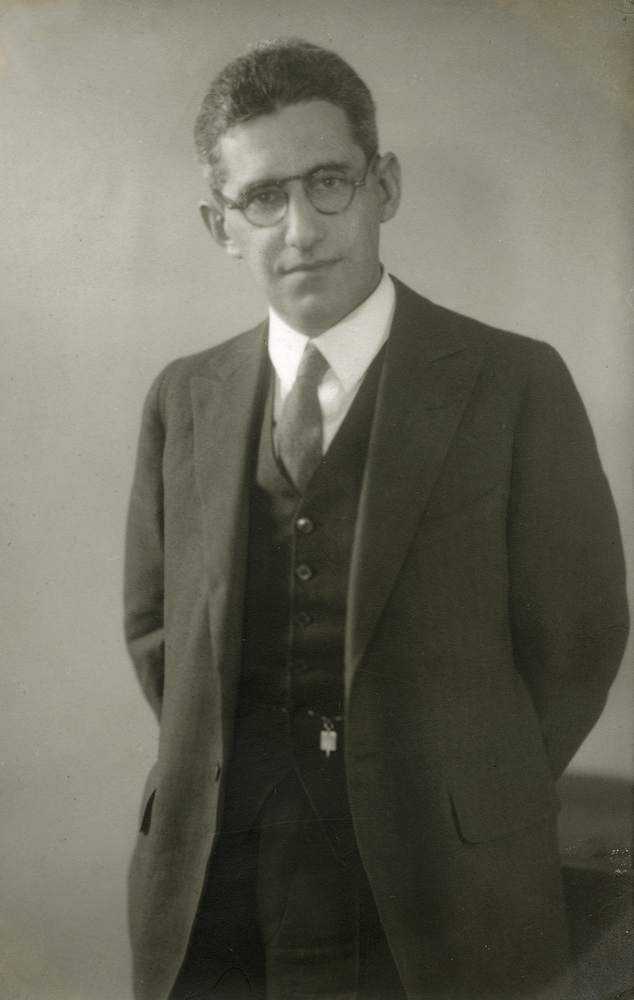
\includegraphics[width=.95\textwidth]{figures/bloomfield_standing.jpg}
  \caption{Leonard Bloomfield in his 30s}
  \label{fig:ch.bloomfield.bloomfield_standing}
\end{wrapfigure}
More important than the word, of course, is the sort of linguistic
\isi{variation} it refers to, and {\Bloomfield}'s attitude toward
this. `Phonetic change' clearly appears in the 1933 book as a category
of linguistic \isi{variation} distinct from that found among the alternants
of a single \isi{phoneme}: such ``change in the primary phonemes of a form''
is put on a par with other concomitants of ``the meaningful
arrangements of forms in a language,'' i.e., ``its \emph{grammar}'':
\emph{order} (the sequence in which the constituents of a complex form
are arranged); \emph{modulation} (the use of secondary phonemes of
\isi{stress}, \isi{pitch}, etc.); and \emph{selection} (the simple choice of one
form rather than another). {\Bloomfield}'s discussion of morphology in
chapters 13 and 14 of \textsl{Language} treats a great deal of the
\isi{variation} that would be called morphophonemic by later writers. It is
clear that this \isi{variation} is dealt with as \isi{alternation} between
distinct phonemic forms, and not as \isi{alternation} between distinct
realizations of the same phonemic form.

The first systematic treatment of \isi{morphophonemics} in {\Bloomfield}'s work
is \citealt{bloomfield:menomini_morphophonemics}, his classic paper on
\ili{Menomini}.\footnote{Although this paper, together with
  \citealt{swadesh.voegelin39:alternation} from the same year, is
  often taken to provide the beginnings of \isi{morphophonemics} in American
  linguistics, \citet[278]{hymes83:hist.ling.anthro} argues that
  ``American abstract \isi{morphophonemics} would seem to have its origin in
  the "First Yale School" in the post-doctoral collaboration about
  1933-36 of {\Newman} and {\Swadesh} with {\Sapir}.'' See
  section~\ref{sec:struct-morphophonemics} in the following chapter
  for further discussion.} Here the fundamental methodology of such
descriptions is described with clarity:

\begin{quotation}
  The process of description leads us to set up each morphological
  element in a theoretical \emph{basic} form, and then to state the
  deviations from this \isi{basic form} which appear when the element is
  combined with other elements. If one starts with the basic forms and
  applies our statements \ldots\ in the order in which we give them,
  one will arrive finally at the forms of words as they are actually
  spoken. Our basic forms are not ancient forms, say of the
  \ili{Proto-Algonquian} parent language, and our statements of internal
  sandhi are not historical but descriptive, and apply in a purely
  \emph{descriptive order}. However, our basic forms do bear some
  resemblance to those which would appear in a description of
  \ili{Proto-Algonquian}, some of our statements of \isi{alternation} \ldots\
  resemble those which would appear in a description of
  \ili{Proto-Algonquian}, and the rest \ldots, as to content and order,
  approximate the historical development from \ili{Proto-Algonquian} to
  present-day \ili{Menomini}.
  \citep[109f.]{bloomfield:menomini_morphophonemics}
\end{quotation}

A morphophonemic description, then, starts from a ``theoretical basic
form,'' and applies to this a series of rules modifying its shape. ``The
forms now arrived at are phonemic forms of the actual \ili{Menomini}
language. \ili{Menomini} phonetics, however, allows a great deal of latitude
to some of its phonemes, and of some \isi{overlapping} between phonemes''
\citep[115]{bloomfield:menomini_morphophonemics}. The description of
this subphonemic \isi{variation} is the responsibility of a different part
of the grammar, namely, the principles defining the phonetic
realizations of phonemes.

These ``theoretical basic forms'' are made up largely of phonemic
elements, but also include some additional abstract units. For
example, in \ili{Menomini} there is a rule by which \emph{n} is replaced by
\emph{s} under certain circumstances. A large number of \emph{n}'s are
not subject to this change, however, and these {\Bloomfield} writes as
\emph{N} in basic forms. The morphophonemic element \emph{N} is
everywhere replaced by \emph{n}; it corresponds not to a distinct
\isi{phoneme}, but rather to instances of \emph{n} whose behavior with
respect to the \isi{alternation} in question is unusual. Several other
distinct morphophonemic symbols are introduced in the \ili{Menomini}
description for vowels whose behavior with respect to one or another
\isi{alternation} is not the usual one; these are all converted to normal
phonemic vowels before the end of the derivation.

This overall technique of morphophonemic description was largely
derived from that of Pāṇini's grammar of \ili{Sanskrit}. {\Bloomfield} was well
acquainted with Pāṇini's work from his early education in
\ili{Indo-European}; he described it in a 1929 review as ``one of the
greatest monuments of human intelligence and (what concerns us more)
an indispensable model for the description of languages''
\citep[219]{hockett70:bloomfield.anthology}. As we remarked above, it
is possible to suggest that the \emph{saṁjña} rules of Pāṇini's
\emph{Aṣ̣ṭ̣ādhyāyī} (cf. \citet[ch. 6]{kiparsky79:panini}, for a
description of these), and not {\Weiss}'s postulates for psychology,
furnished the actual substantive inspiration for
\posscitet{bloomfield26:postulates} attempted axiomatization of
linguistics.

The rules of a morphophonemic description are motivated by the need to
treat alternations among phonemically distinct forms of the same
grammatical element in a systematic way. A language with no
alternations would have no \isi{morphophonemic rules}, and there would be no
reason to establish a theoretical \isi{base form} for any grammatical
element that differed from its surface phonemic form.

Internal to the set of rules, \citet[210f.]{bloomfield:lg} also
assumes at least the outline of a classification, even before the
\ili{Menomini} paper. Alternations can be \emph{phonetic} if they relate
alternants that differ in terms of phonetic modification (change in a
limited number of phonetic properties, as with the variants [-s],
[-z], and [-ez] of the \ili{English} \isi{regular} plural) rather than wholesale
replacement (e.g., the \isi{alternation} between the \isi{regular} plural endings
and [-en] in \emph{oxen}). They may independently be classified as
\emph{regular}, when some linguistically recognizable characteristic
of the environment conditions the \isi{alternation}, as opposed to
alternations conditioned by an arbitrary set of forms; again, the
plural ending of \emph{oxen} serves as an example of an irregular
\isi{alternation}, since there is no linguistically relevant property of
\emph{ox} that conditions the ending [-en]. Finally, an \isi{alternation} is
\emph{automatic} if it is \isi{regular} and conditioned by the phonological
structure of the environment as opposed to grammatically conditioned
alternations (a notion that will later be taken up by
\citet{wells49:automatic}, see section~\ref{sec.struct.interaction}).

The bulk of the rules in {\Bloomfield}'s morphophonemic descriptions
represent automatic alternations. Though these may well have some
specified (arbitrary) exceptions, they are regularly conditioned in
terms of the morphophonemic environment. In fact, the use of distinct
symbols for morphophonemes is motivated by the desire to render as
many alternations as possible automatic in this sense.

To this end also, many items are set up in theoretical shapes that
differ from the form they take in isolation. Thus, final consonant
clusters are set up in \ili{Menomini} forms in order to account for the
shape stems show when followed by further endings, despite the fact
that all such clusters are reduced to a single consonant phonetically
in final position. Some sequences of segments are established
underlyingly which cannot ever occur in surface forms. For instance,
-w- is always lost in the semivowel sequence -wy- after a consonant;
this representation is used to describe those instances of -y- that do
not cause \isi{palatalization} of a preceding consonant. Such analyses show
that {\Bloomfield} definitely did not adhere to the constraint discussed
in chapter~\ref{ch.sapir} on {\Sapir}'s underlying forms (including also
his positing of underlying stem-final \isi{consonants} in \ili{Samoan} verbs, as
discussed in the appendix to that chapter). Purely diacritic
distinctions are also set up, in which two or more underlying forms
have the same surface realization but different phonological behavior.

In addition to formulating the description so that as many rules as
possible will be automatic alternations, {\Bloomfield} also formulates
individual rules in as general as possible a fashion, rather than
limiting himself to attested instances of their application. For
example, he states a rule by which all sequences of postconsonantal
semivowels contract with a following vowel other than \emph{a} or
\emph{ā}. Statements of the particular contraction products are
subordinated to this general rule, and he also notes that no instances
of the contraction of \emph{y} with \emph{ō, o} are attested—showing
that the rule is actually more general than necessary.

In at least one instance, this desire to maximize the generality of
particular rules even leads {\Bloomfield} to violate the basic principle
that phonemic analysis should show all \emph{and only} the distinctive
properties of segments. In \ili{Menomini}, there is a rule by which long and
short \emph{e} and \emph{o} are raised to \emph{i} and \emph{u},
respectively, when a high vowel or semivowel follows later in the word
(with some added complications that are irrelevant
here). Interestingly, this rule is the only source of phonetic [ū] in
the language. Properly speaking, then, \emph{ū} should not be treated
as a \isi{phoneme} in \ili{Menomini} but as a variant of \emph{ō}. If this were
done, however, the rule in question could not be stated in its full
generality, since the output of the \isi{morphophonemic rules} is supposed
to be a sequence of phonemes, not variants. The morphophonemic rule
should thus be stated so as to apply to \emph{e}, \emph{ē}, and
\emph{o}, but not \emph{ō}; and then a distinct rule should be stated
to convert phonemic \emph{ō} to phonetic [ū] under the identical
conditions.

This is of course a perfect example of the argument Halle would later
adduce against the linguistic appropriateness of a `taxonomic'
phonemic level, which we have already mentioned in
chapter~\ref{ch.prague} above and to which we will return in
chapter~\ref{ch.genphon}.\footnote{\citet{bever67:thesis} provides an
  account of {\Bloomfield}'s descriptions of \ili{Menomini} in the terms of
  early Generative Phonology. He maintains (pp. 51ff.) that {\Bloomfield}
  saw the consequences of this argument and explicitly rejected an
  independent level corresponding to phonemics. This interpretation
  seems rather strained to me, and {\Bloomfield}'s efforts to evade the
  issue as described here would seem to confound it.} {\Bloomfield} quite
recognized the problem presented by this example and took two
different lines of approach toward it. In his
\citeyear{bloomfield:menomini_morphophonemics} presentation of
\ili{Menomini}, he states (on this basis) that since ū occurs only in this
\isi{alternation}, it ``is not a full \isi{phoneme}.'' In his presentation of
``actual \ili{Menomini} phonemes,'' he includes ū but puts it in parentheses
(a unique status) and refers to it (without further \isi{explanation}) as a
``semi-\isi{phoneme}.''

By {contrast}, in \textsl{The \ili{Menomini} Language},
\citet{bloomfield62:menomini} includes \emph{ū} in the list of
phonemes without comment or parentheses. Later, he discusses its
special status, but argues that it should be treated as a \isi{phoneme}
anyway: ``In this \isi{alternation}, however, the difference of \emph{o:} and
\emph{u:} is parallel with that of \emph{e:} and \emph{i:}, two sounds
which unmistakably figure as separate phonemes. Moreover, this
difference of \emph{o:} and \emph{u:} is maintained by persons in
whose speech the \isi{alternation} has lost its regularity. Also, there are
a few interjections in which \emph{u:} (and never \emph{o:}) is used:
\emph{capu:q} `splash!', \emph{ku:h} `stop it!'. A \isi{contrast} of
\emph{o:} and \emph{u:} appears in the foreign words \emph{co:h} `Joe'
and \emph{cu:h} `Jew''' \citep[5]{bloomfield62:menomini}.

The arguments for the phonemic status of \emph{ū} thus reduce to: (a)
the generality of the \isi{alternation}, which would be destroyed if [ū]
were treated as it otherwise should be, i.e., as nonphonemic; (b) the
probable phonemic status of the vowel in marginal idiolects which have
lost the \isi{regular} morphophonemic rule; and (c) the appearance of
unconditioned ū in a few expressive forms and foreign
borrowings. Clearly none of these arguments (except possibly the last)
really bear on the phonemic status of [ū], which would undoubtedly
have been treated as a mere variant if it were not for the necessity
to state the \isi{alternation} as a unitary generalization.

Numerous other aspects of morphophonemic description would have to be
explored in order to arrive at a complete understanding of
{\Bloomfield}'s practice.  Chapter 13 in \textsl{Language}, for example,
devoted to morphology, treats at considerable length the issue of how
basic forms are to be arrived at. As one would imagine from the
importance he attaches to generality of rules, the primary
consideration is to choose a representation from which all alternating
variants can be produced by means of rules of automatic
\isi{alternation}. Often this is one of the occurring variants of the
alternating form, though perhaps not the one that appears in
isolation. For example, he indicates a distinction in \ili{Russian} between
voiced and voiceless final obstruents which is neutralized in the
unextended form; he posits Sāmoan verb stems with underlying final
\isi{consonants} which are always deleted when no suffix follows, and
similarly he sets up \ili{Menomini} forms with final clusters that are
generally simplified unless suffixed.

Frequently, it is not considerations internal to the alternating form
that motivate the decision on a basic shape but, rather, aspects of
the rules involved. For example, {\Bloomfield} considers the forms of the
\isi{regular} plural in \ili{English}, and concludes that [ez] should be taken as
basic (rather than [s] or [z]) because a rule is necessary in any case
to delete the vowel in contracted forms of the copula \emph{is} (e.g.,
\emph{Jack's coming}), and the same rule can be extended to the plural
(for criticism of this argument, see
\citealt{sra73:english-inflection}). Considerations of rule generality
sometimes lead {\Bloomfield} to take as basic a shape that is not usually
thought to be `basic' in some other sense: thus, he takes the basic
form of \ili{French} adjectives to be the feminine, since the masculine can
be derived from that by a simple rule of final consonant deletion.

Other principles can also be found behind {\Bloomfield}'s practice which
determine the way his descriptions are organized. For example,
\citet{kenstowicz75:application} finds reasons, developed in greater
detail by \citet{miner81:bloomfield}, to believe that {\Bloomfield}'s
rules are stated so as to lead to derivations that minimize the
`\isi{opacity}' of forms in roughly the sense of
\citet{kiparsky:3dimensions}. Miner\ia{Miner, Kenneth} also argues that {\Bloomfield}'s
rules are sometimes more complex than they would otherwise need to be
in order to minimize the need for artificial intermediate stages of a
derivation.

We do not go further into these issues here, however, because they
have little or no bearing on {\Bloomfield}'s actual theory of the
phonological structure of language. This may seem contradictory, but
in fact there is good reason to believe that such principles as one
can uncover in his morphophonemic practice would have been attributed
by {\Bloomfield} to the activity of linguists, rather than to the nature
of language. This of course is quite contrary to the practice in
phonology today, where claims about the organization of linguist's
grammars are intended to be interpreted as claims (in some sense)
about the structure of natural language.

{\Bloomfield} clearly believed that \isi{phonemic representations}, and the
relation between them and phonetic realization, correspond to
something `real' about a language. The status of alternations and
their description in morphophonemic terms, however, is somewhat
different. {\Bloomfield} was certainly of the opinion that the relation
between alternating forms was a real one: alternating forms that
differ phonemically are still variants of the same grammatical
element. The status of the \isi{morphophonemic rules} that describe the
relation is nonetheless dubious. ``What is here involved is not merely
our convenience, but the speakers' habit of correlating morphological
complexes. To be sure, we take the liberty of inventing a basic
(morphophonemic) formula and then telling how it is to be modified to
produce the actual (phonemic) utterance, but this is merely a
descriptive device'' (from a letter to {\Hockett} quoted in
\citealt[371]{hockett70:bloomfield.anthology}). The correlation of
actual phonemic forms in \isi{alternation} here is `real,' but this is a
matter of morphology rather than of phonology. As for the
morphophonemic mechanics by which we describe that correlation, ``this
is not a question about the language: it is a question about the
clearest and most convenient way of telling about the language''
(another letter to Hockett quoted in
\citealt[375]{hockett70:bloomfield.anthology}).

While {\Bloomfield} was certainly one of the most noteworthy early
practitioners of the morphophonemic method of description, (which he
had learned from Pāṇini's grammar), we should not therefore make the
anachronistic assumption that he understood such descriptions in the
same way later linguists do. In particular, he seems clearly to have
considered them in the same light as he did Pāṇini's description: an
elegant artifact, providing a uniform and concise account of a complex
set of facts, but not to be confused with the actual language capacity
of speakers. Only the phonemic forms, and the morphological fact of
relations between them, could be considered to have that status. For
{\Bloomfield}, the beginning and the end of a theory of phonological
structure in natural language was a theory of phonemic
\isi{representations}.

%%% Local Variables: 
%%% mode: latex
%%% TeX-master: "/Users/sra/Dropbox/Docs/Books/P20C_2/LSP/main.tex"
%%% End: 
